\chapter{First Chapter SfS Template} 

\section{To include a picture}
%% picture 'h'ere, 'b'ottom or 't'op; '!' try to impose your will on latex
\begin{figure}[hbt!]
  %% no file extension; .85 stands for 85% of text width
  \epsfCfile{.85}{geys-2kern} 
  %% legend for the list of figures at the beginning of you thesis
  \caption[Geyser data: binned histogram, Silverman's and another kernel]
  %% legend displayed below the graph.
  {Old Faithful Geyser eruption lengths, $n=272$; binned data and two
    (Gaussian) kernel density estimates ($\times 10$) with $h=h^*= .3348$
    and $h= .1$ (dotted).}
  \label{fig:geys1}
\end{figure}

Or also with \texttt{includegraphics}:
%% picture 'h'ere, 'b'ottom or 't'op; '!' try to impose your will on latex
\begin{figure}[hbt!]
  \centering
  %% no file extension; .5\textwidth stands for 50% of text width
  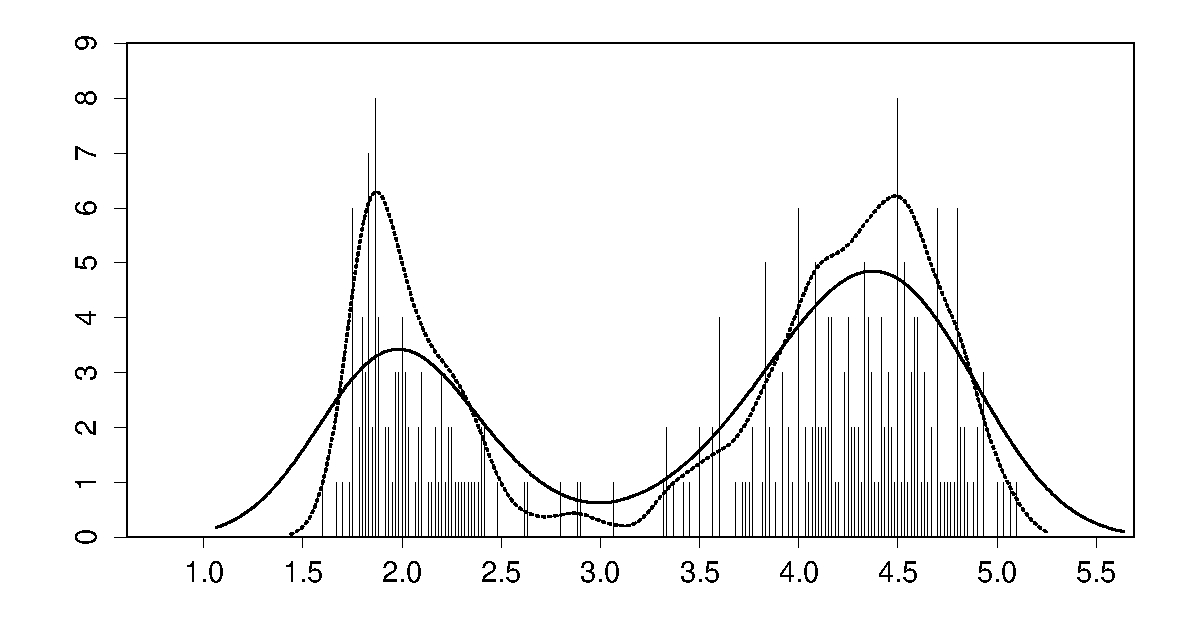
\includegraphics[width=.5\textwidth]{geys-2kern}
  %% legend for the list of figures at the beginning of you thesis
  \caption[Geyser data: binned histogram, Silverman's and another
  kernel]
  %% legend displayed below the graph.
  {Old Faithful Geyser eruption lengths, $n=272$; binned data and two
    (Gaussian) kernel density estimates ($\times 10$) with $h=h^*= .3348$
    and $h= .1$ (dotted).}
  \label{fig:geys2}
\end{figure}

\section{To make a proof}
\begin{proof}
  $1 + 1 = 2$
\end{proof}

\section{To include \Rp code}
See information in Appendix~\ref{app:complement}.


\section{Other information}
Put a text between quotes: make sure to use nice quotes, such as ``quote''.

Cite a document in the bibliography (an example here): \cite{Gelman2008}.
Or mention that \citeauthor{Konis2007} (a person) or \citeauthor{Hastie2009} (multiple
persons) have already done quite a bit work.

Referencing a different part of your work: please refer to Appendix \ref{app:complement}.
